%biafra ahanonu
%LaTeX_Boilerplate
%updated: 2012.12.01

\ffigure{Images/Map.jpg}{6in}{Map}{Map of Civilizations Discussed}{Image of the Americas with locations of the cultures discussed in the text. We start with the Algonquin and then discuss the Cahokia, Hisatsinom, Olmec, Maya, Aztec, Chavin, Inca, and Tehuelche.}{p!}

\begin{figure*}[ht!]
	\begin{center}
		\subfloat[Three Sisters]{\includegraphics[width=3.0in]{Images/threesisters.jpg}}  
		\subfloat[Corn God, Centeotl]{\includegraphics[width=3.0in]{Images/corngod.jpg}} \\
		\subfloat[North American Game]{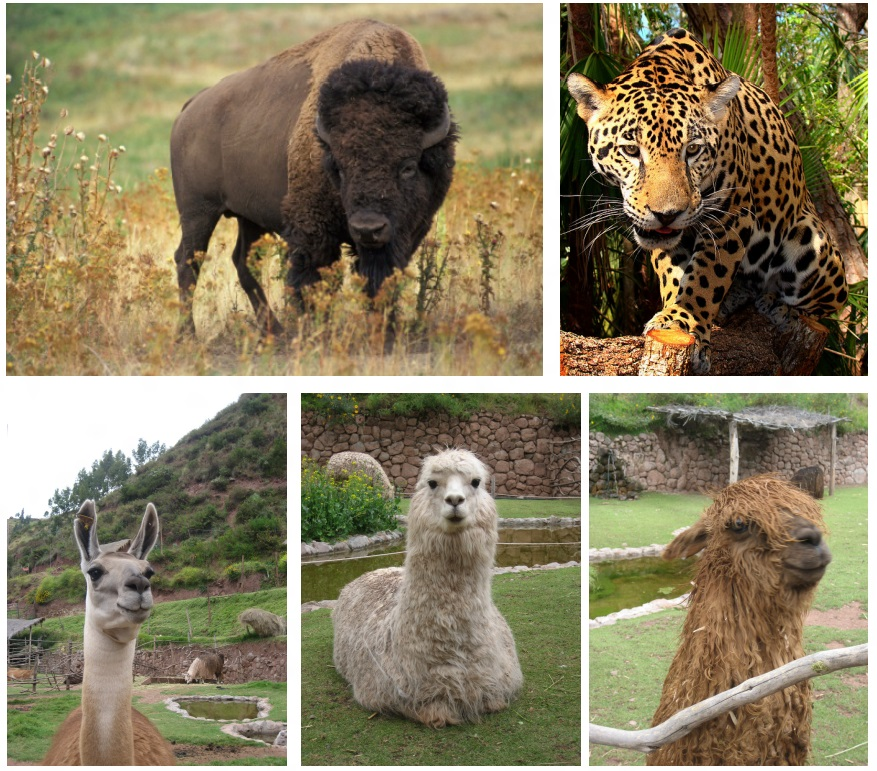
\includegraphics[width=3.0in]{Images/nagame.jpg}} 
		\subfloat[Cenote, Yucatan]{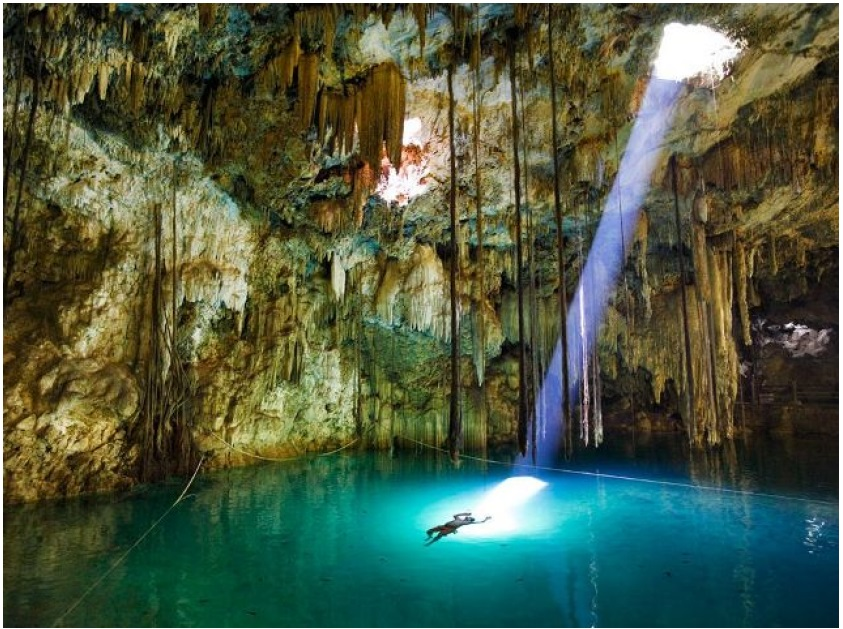
\includegraphics[width=3.0in]{Images/cenote.jpg}}
		\captionsetup{labelformat=empty}
		\caption{\textbf{Figure \ref{fig:1} |  Early native American staples}\\ a, the three sisters that enabled stable crop integration. b, the corn god of the Aztecs, recognizing the importance of the crop. c, the different type of game hunted in the Americas. d, the cenote, which were seen as sacred by the Maya.}
		\label{fig:1}
	\end{center}
\end{figure*}